\section{Introduction}
\begin{itemize}
    \item What is the problem? Illustrate with an example.
\end{itemize}

\todo[inline]{Example Haskell Data Type}
\todo[inline]{Calculate a result over the Data Type}
\todo[inline]{Cache the incremental computation over the data type}

\begin{haskell}
data Tree = Leaf Int
          | Node Tree Int Tree 
\end{haskell}

The problem is called the \textbf{binary tree maximum path sum}.

\begin{haskell}
exampleTree :: Tree    
exampleTree = Node (Node (Leaf 8) 7 (Leaf 9)) 3 (Node (Leaf 5) 4 (Leaf 2))
\end{haskell}

\begin{figure}[H]
    \centering
    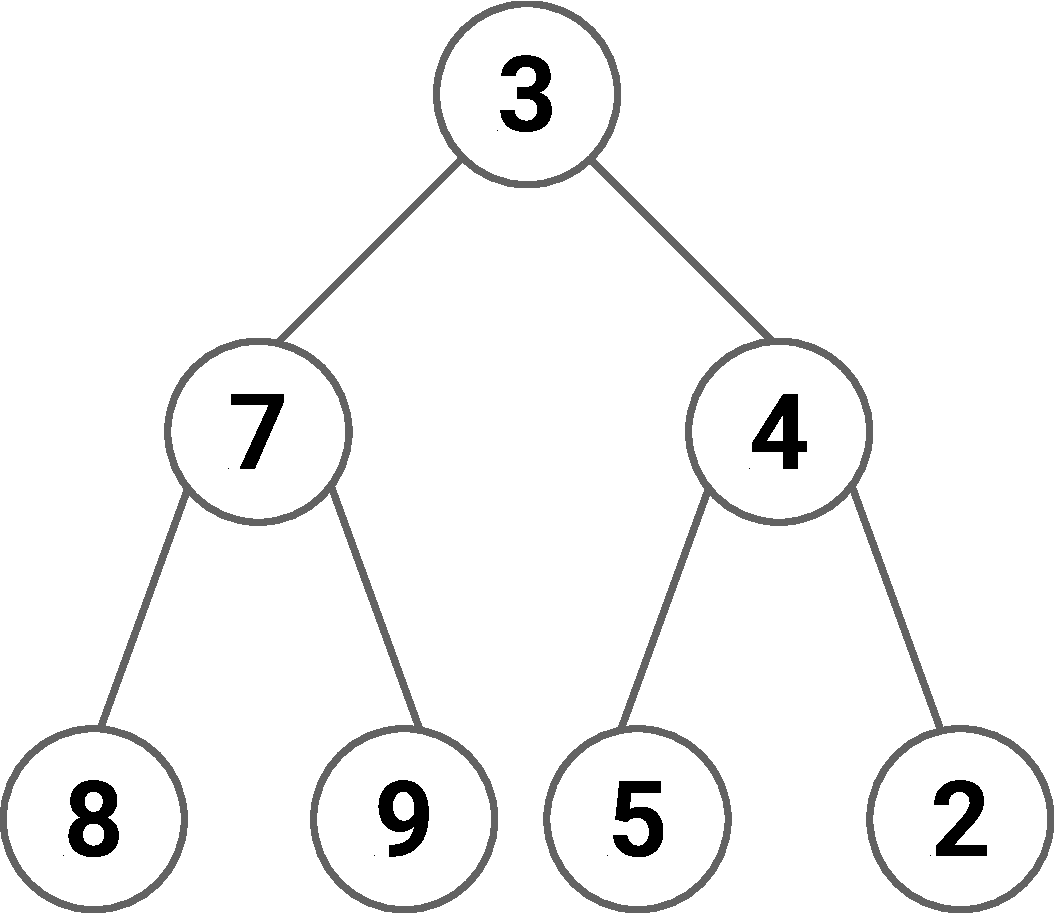
\includegraphics[width=.4\textwidth]{Tree.pdf}
    \caption{Graphic visualization of the \texttt{exampleTree}}
\end{figure}

\todo[inline]{This function does not work for negative values}
\begin{haskell}
maxPathSum :: Tree -> Int
maxPathSum (Leaf x)     = x
maxPathSum (Node l x r) = x + max (maxPathSum l, maxPathSum r)

maxPathSum exampleTree !$\equiv$! 19
\end{haskell}

\begin{figure}[H]
    \centering
    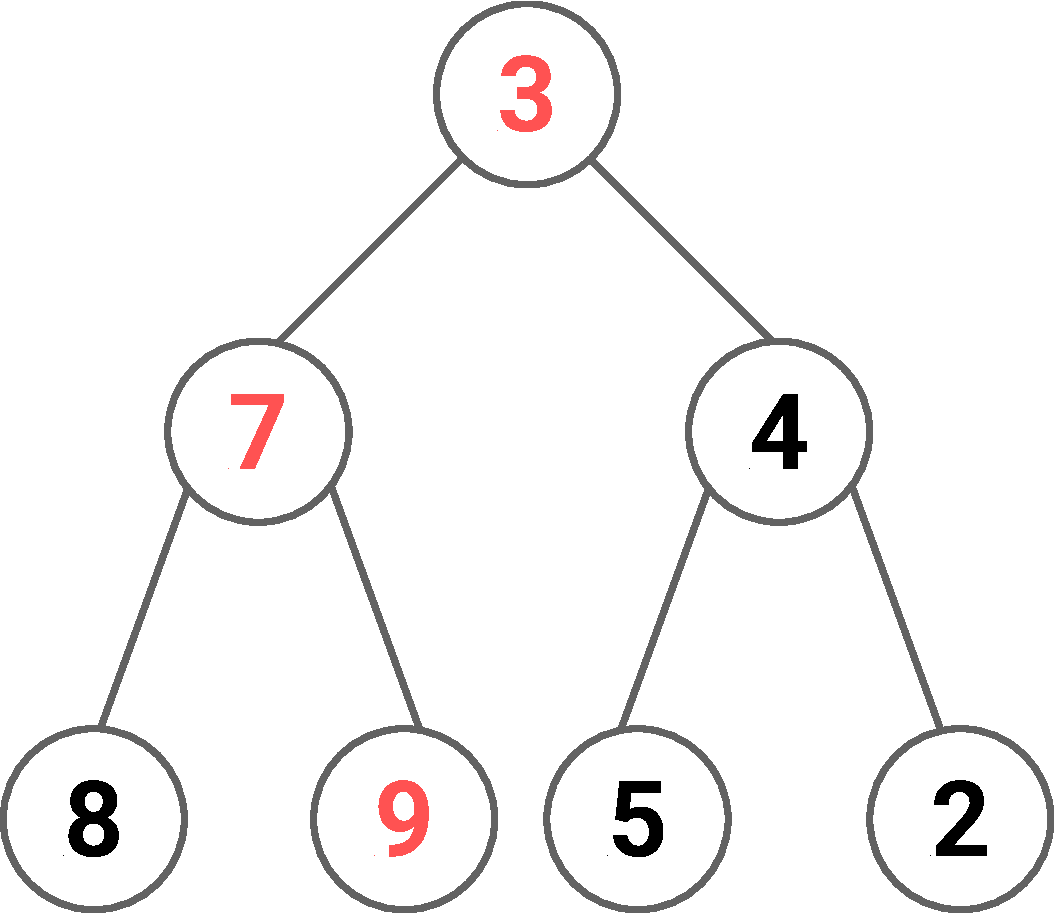
\includegraphics[width=.4\textwidth]{SolvedTree.pdf}
    \caption{The path for the maximum sum}
\end{figure}

\begin{haskell}
data MerkleTree = LeafH Hash Int
                | NodeH Hash Tree Int Tree

merkle :: Tree -> MerkleTree
merkle (Leaf x)     = LeafH (hash ["Leaf", x]) x
merkle (Node l x r) = NodeH (hash ["Node", x, hl, hr]) nl x nr
  where
    nl@(NodeH hl _ _ _) = merkle l
    nr@(NodeH hr _ _ _) = merkle r
\end{haskell}

\begin{figure}[H]
    \centering
    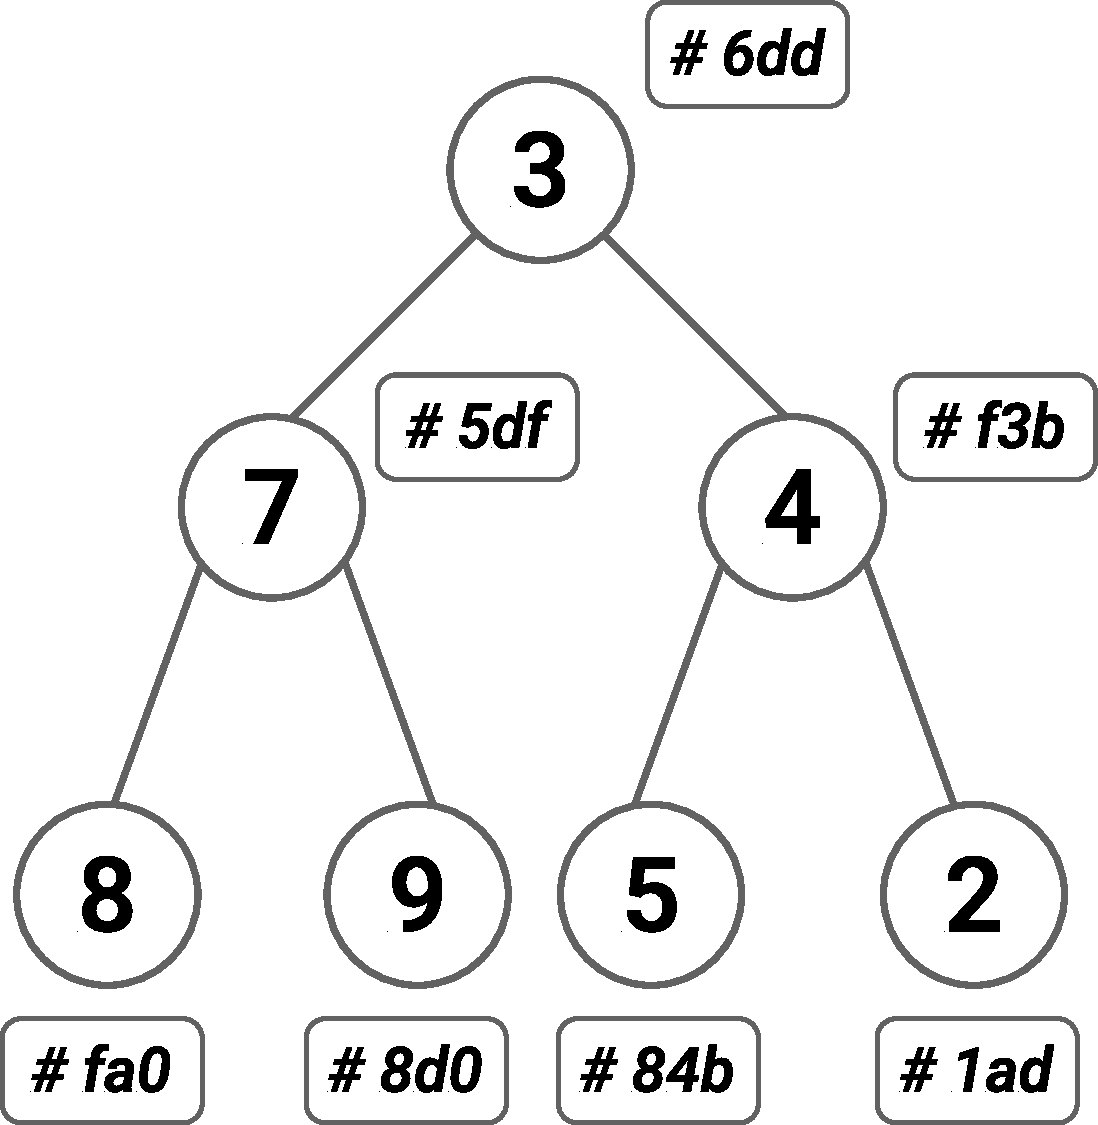
\includegraphics[width=.4\textwidth]{MerkleTree.pdf}
    \caption{The \texttt{MerkleTree} of exampleTree}
\end{figure}

\begin{haskell}
maxPathSumInc :: MerkleTree -> (Int, Map Hash Int)    
maxPathSumInc (LeafH h x)     = (x, insert h x empty)
maxPathSumInc (NodeH h l x r) = (y, insert h y (ml <> mr))  
  where
    y = x + max (xl, xr)
    (xl, ml) = maxPathSumInc l
    (xr, mr) = maxPathSumInc r
\end{haskell}

\begin{figure}[H]
    \begin{minipage}[c]{0.55\textwidth}
        \centering
        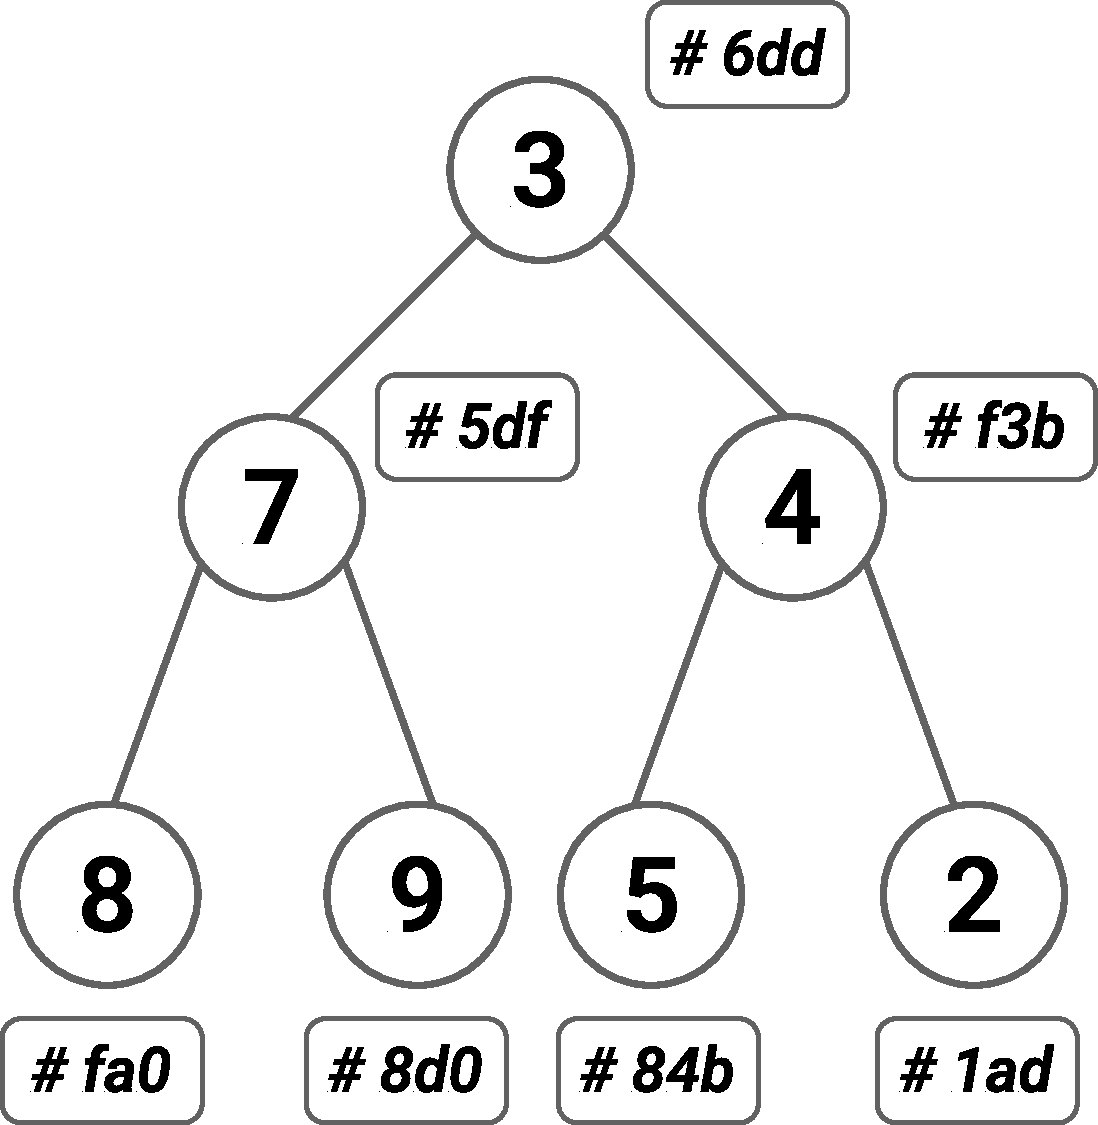
\includegraphics[width=.7\textwidth]{MerkleTree.pdf}
    \end{minipage}
    \hspace{0.1\textwidth}
    \begin{minipage}[c]{0.35\textwidth}
        \centering
        \begin{tabular}{|l|r|}
            \hline
            \textbf{Hash Nodes} & \textbf{Max Sum} \\
            \hline
            \# 6dd & 19 \\
            \hline
            \# 5df & 16 \\
            \hline
            \# fa0 & 8 \\
            \hline
            \# 8d0 & 9 \\
            \hline
            \# f3b & 9 \\
            \hline
            \# 84b & 5 \\
            \hline
            \# 1ad & 2 \\
            \hline
        \end{tabular}
    \end{minipage}
    \caption{The \texttt{MerkleTree} with intermediate results}    
\end{figure}

\begin{figure}[H]
    \centering
    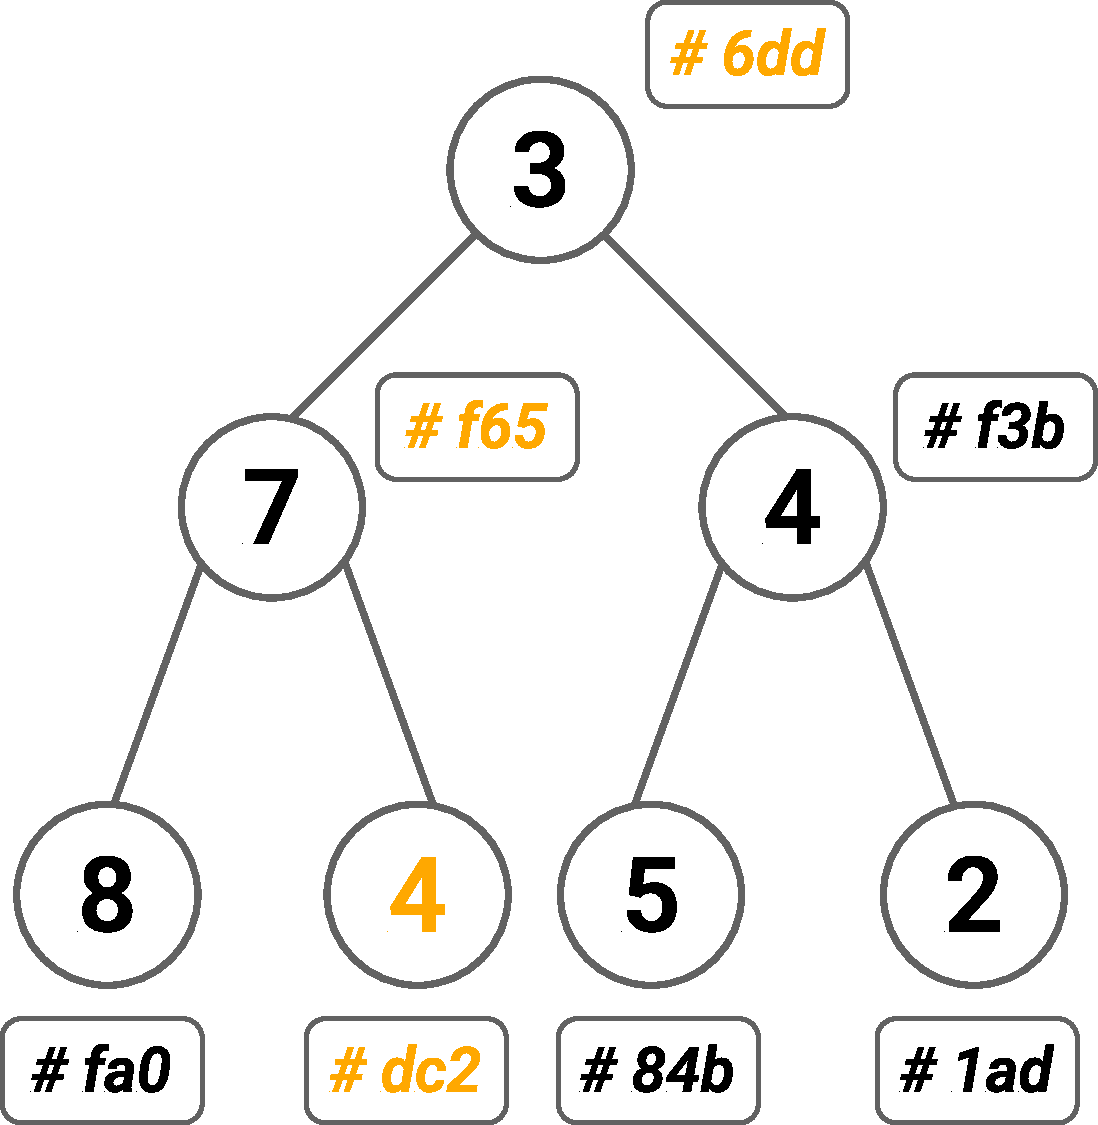
\includegraphics[width=.4\textwidth]{ChangedMerkleTree.pdf}
    \caption{Changed Tree}
\end{figure}

\begin{haskell}
maxPathSumMap :: Map Hash Int -> MerkleTree -> (Int, Map Hash Int)
maxPathSumMap m (LeafH h x) = case lookup m h of
  Just y  -> (y, m)
  Nothing -> (x, insert h x m)
maxPathSumMap m (NodeH h l x r) = case lookup m h of
  Just y  -> (y, m)
  Nothing -> (y, insert h y (ml <> mr))
    where
      y = x + max (xl, xr)
      (xl, ml) = maxPathSumMap m l
      (xr, mr) = maxPathSumMap m r  
\end{haskell}

\begin{haskell}
class (Functor f) => Merkelize f where
    merkle :: Fix f -> Fix (f :*: K Hash)
\end{haskell}

\begin{haskell}
cataMerkle :: (Merkelize f) => (f a -> a) -> Fix (f :*: K Hash) -> (a, Map Hash a)
\end{haskell}

\footnote{The source code is on GitHub at \hyperlink{https://github.com/jortvangorkum/memo-cata}{https://github.com/jortvangorkum/memo-cata}}

\subsection{Contributions}
\begin{enumerate}[label={(\Alph*)}]
    \item A library needs to be implemented which contains the generic \texttt{merkle}, \texttt{cataMerkle} and \texttt{cataMerkleWithMap} functions
\end{enumerate}

\subsection{Research Questions}
Using the previously mentioned library, there is a multitude of questions to be answered:
\begin{enumerate}[label={(\Alph*)}]
    \item What parameters can be tweaked to have the best ratio of performance and memory usage?
    \item What type of equivalence is needed to reuse the incremental computation?
    \item What type of data structures are the best for storing the incremental computation?
    \item Could the library be used to perform static analysis in a more performant manner?
\end{enumerate}